% Options for packages loaded elsewhere
\PassOptionsToPackage{unicode}{hyperref}
\PassOptionsToPackage{hyphens}{url}
%
\documentclass[a4paper, 12pt]{article}
\usepackage{amsmath,amssymb}
\usepackage{lmodern}
\usepackage{iftex}
\ifPDFTeX
  \usepackage[T1]{fontenc}
  \usepackage[utf8]{inputenc}
  \usepackage{textcomp} % provide euro and other symbols
\else % if luatex or xetex
  \usepackage{unicode-math}
  \defaultfontfeatures{Scale=MatchLowercase}
  \defaultfontfeatures[\rmfamily]{Ligatures=TeX,Scale=1}
\fi
% Use upquote if available, for straight quotes in verbatim environments
\IfFileExists{upquote.sty}{\usepackage{upquote}}{}
\IfFileExists{microtype.sty}{% use microtype if available
  \usepackage[]{microtype}
  \UseMicrotypeSet[protrusion]{basicmath} % disable protrusion for tt fonts
}{}
\makeatletter
\@ifundefined{KOMAClassName}{% if non-KOMA class
  \IfFileExists{parskip.sty}{%
    \usepackage{parskip}
  }{% else
    \setlength{\parindent}{0pt}
    \setlength{\parskip}{6pt plus 2pt minus 1pt}}
}{% if KOMA class
  \KOMAoptions{parskip=half}}
\makeatother
\usepackage{xcolor}
\usepackage{longtable,booktabs,array}
\usepackage{calc} % for calculating minipage widths
% Correct order of tables after \paragraph or \subparagraph
\usepackage{etoolbox}
\makeatletter
\patchcmd\longtable{\par}{\if@noskipsec\mbox{}\fi\par}{}{}
\makeatother
% Allow footnotes in longtable head/foot
\IfFileExists{footnotehyper.sty}{\usepackage{footnotehyper}}{\usepackage{footnote}}
\makesavenoteenv{longtable}
\usepackage{graphicx}
\makeatletter
\def\maxwidth{\ifdim\Gin@nat@width>\linewidth\linewidth\else\Gin@nat@width\fi}
\def\maxheight{\ifdim\Gin@nat@height>\textheight\textheight\else\Gin@nat@height\fi}
\makeatother
% Scale images if necessary, so that they will not overflow the page
% margins by default, and it is still possible to overwrite the defaults
% using explicit options in \includegraphics[width, height, ...]{}
\setkeys{Gin}{width=\maxwidth,height=\maxheight,keepaspectratio}
% Set default figure placement to htbp
\makeatletter
\def\fps@figure{htbp}
\makeatother
\usepackage[normalem]{ulem}
\setlength{\emergencystretch}{3em} % prevent overfull lines
\providecommand{\tightlist}{%
  \setlength{\itemsep}{0pt}\setlength{\parskip}{0pt}}
\setcounter{secnumdepth}{-\maxdimen} % remove section numbering
\ifLuaTeX
  \usepackage{selnolig}  % disable illegal ligatures
\fi
\IfFileExists{bookmark.sty}{\usepackage{bookmark}}{\usepackage{hyperref}}
\IfFileExists{xurl.sty}{\usepackage{xurl}}{} % add URL line breaks if available
\urlstyle{same} % disable monospaced font for URLs
\hypersetup{
  hidelinks,
  pdfcreator={LaTeX via pandoc}}
\pagestyle{empty} % Removes page number
\usepackage[top=1in, bottom=1in, left=1in, right=1in]{geometry} % Adjust margins

\author{}
\date{}
\begin{document}
\begin{center} % Center-align the content

\includegraphics[width=1.14931in,height=1.35972in]{north-south-university-logo.png}

\textbf{Department of Electrical and Computer Engineering}

\textbf{North South University}

\textbf{\hfill\break SPRING 2024}

\subsection{\uline{Assignment - 1}}
\textbf{\section{ERD Design and Implementation}}

\textbf{\hfill\break\hfill\break
\uline{Submitted By}}

Saif Mohammed

2121913642


\textbf{\hfill\break\hfill\break
\uline{Course Details}}

CSE311 (Section 1)

Database Management Systems

\textbf{\hfill\break\hfill\break
\uline{Submitted To}}

Dr. Abu Sayed Mohammad Latiful Hoque

Professor, Department of Electrical and Computer Engineering

North South University


\textbf{\hfill\break\hfill\break
\uline{Submission Date}}

February 29, 2024
\end{center} % End centering


\newpage
\section{\textbf{\uline{Q1 - ER Diagram (Chen Notation):}}}
\begin{figure}
    \centering
    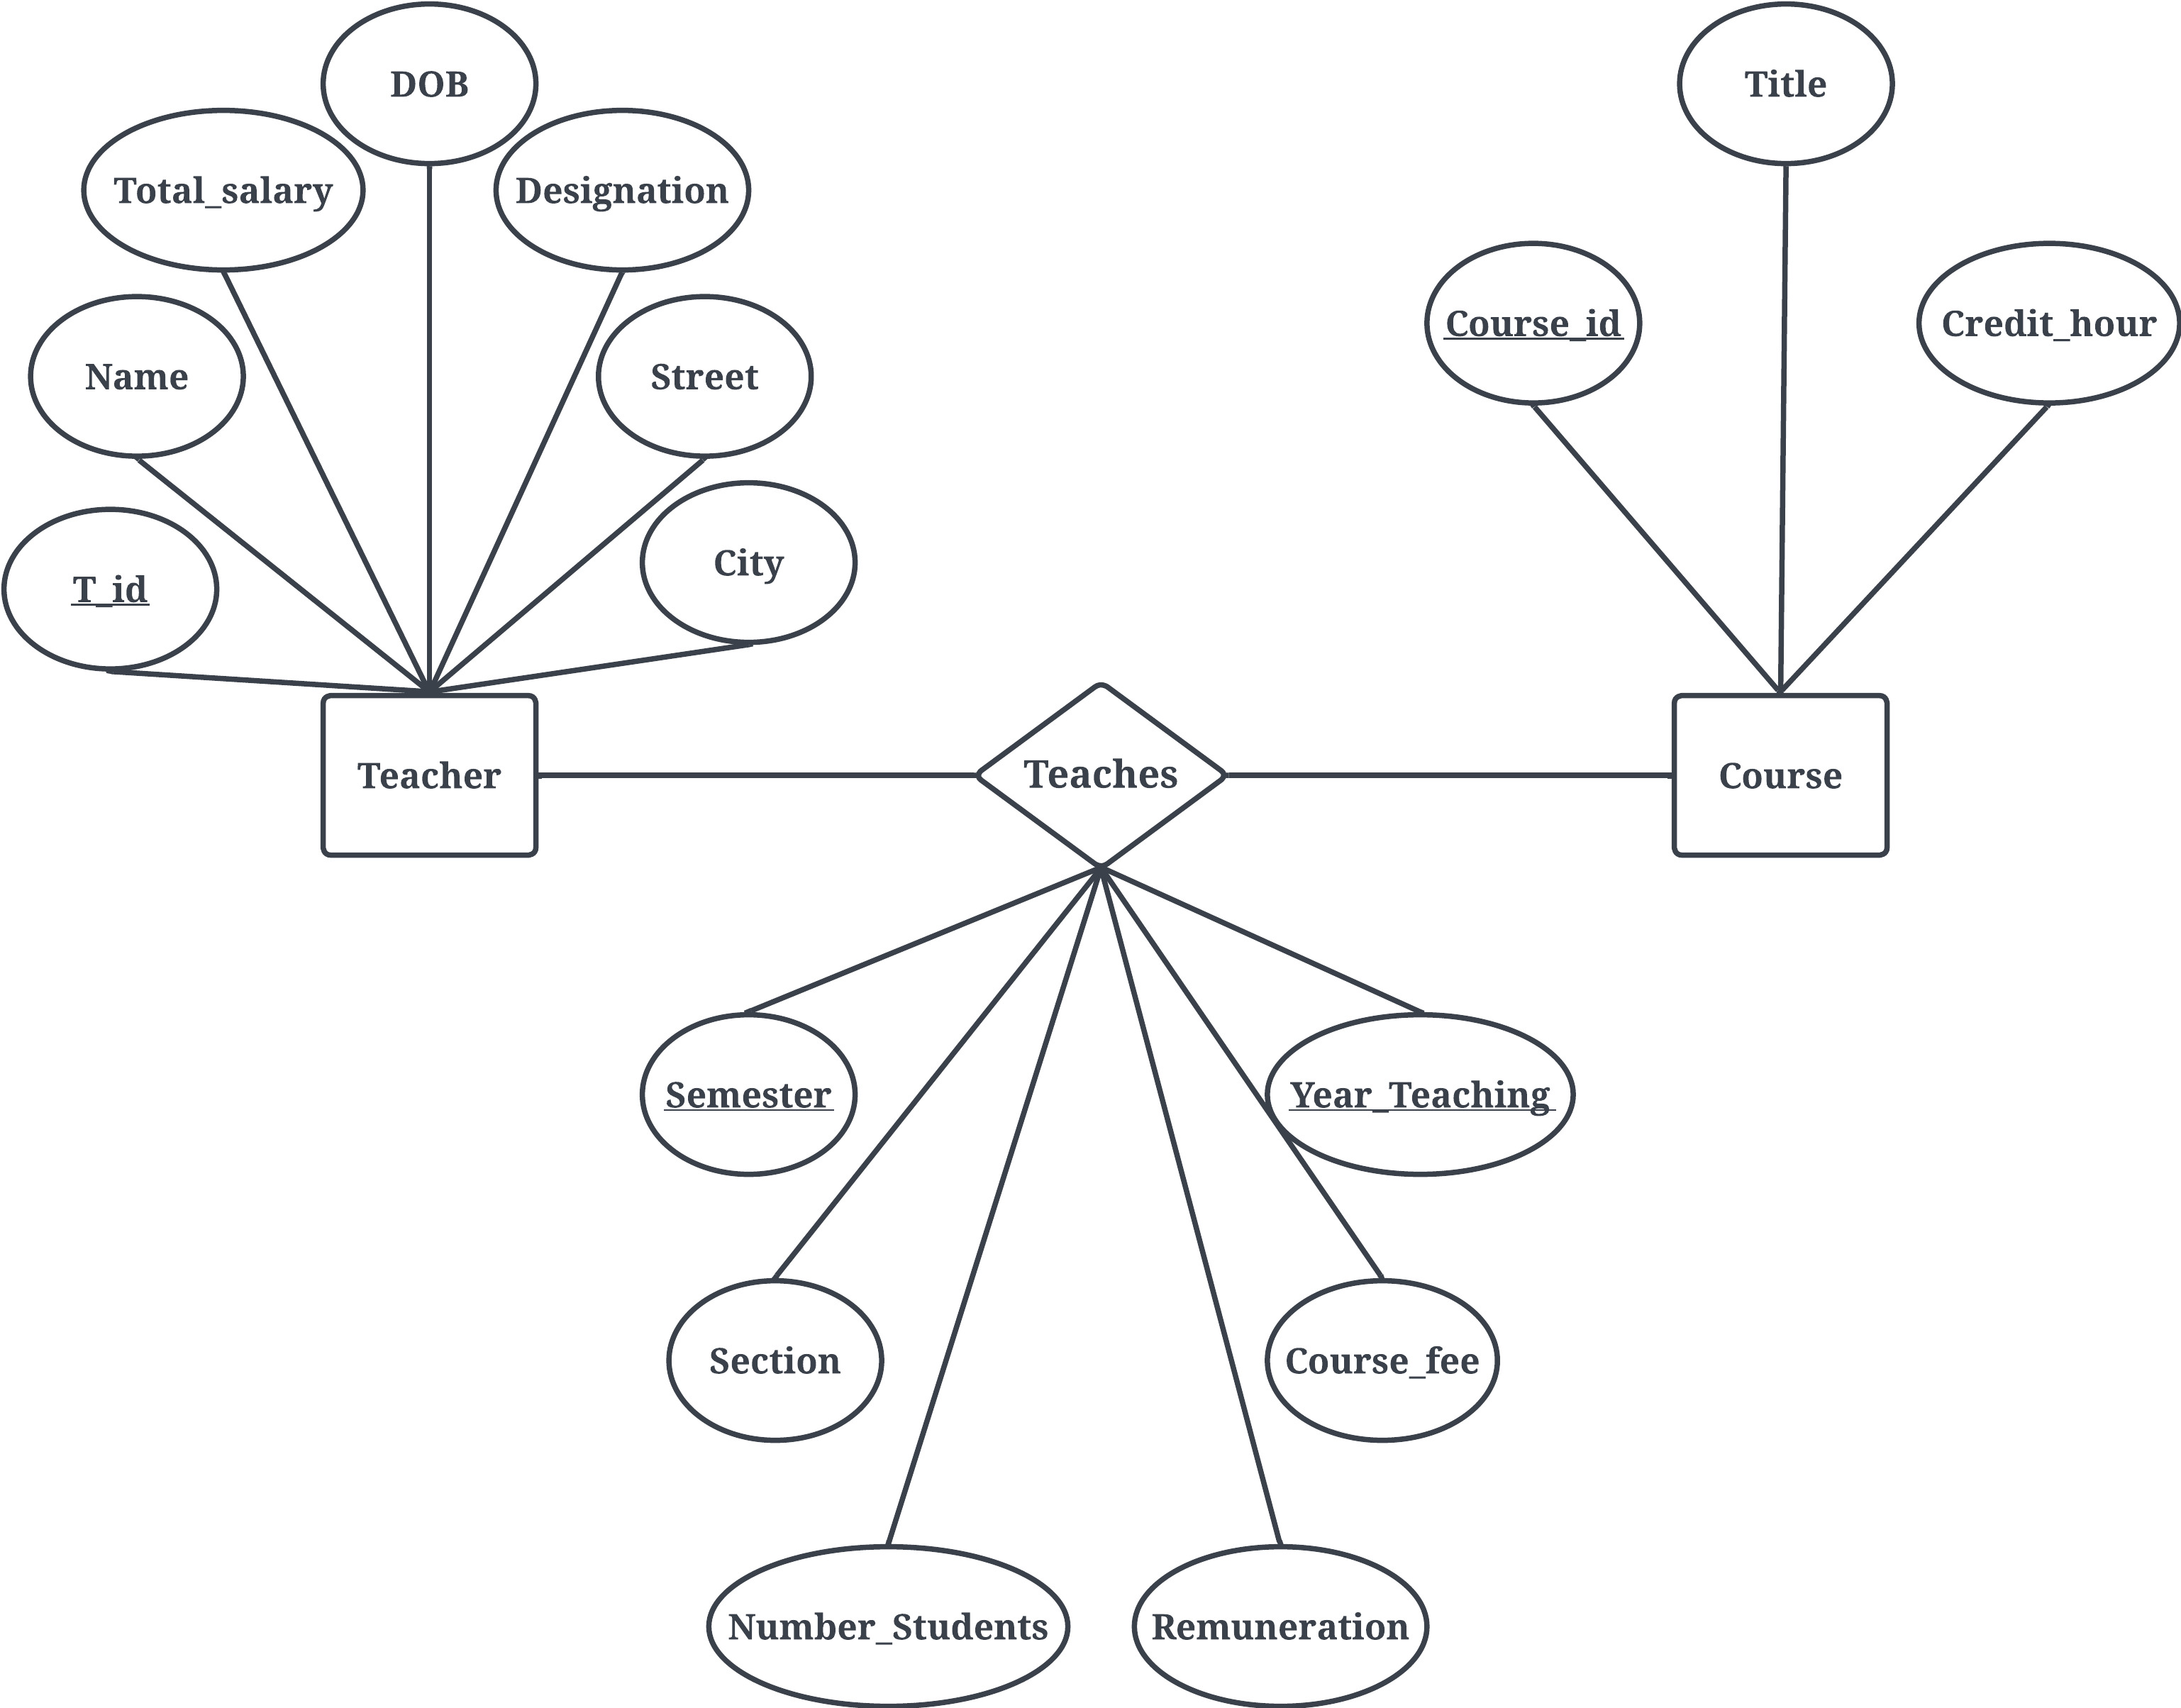
\includegraphics[width=1\linewidth]{Q1.jpeg}
\end{figure}


\section{\textbf{\uline{Q1 - Relation Schema:}}}
Teacher(\uline{T{\_}id}, Name, DOB, Street, City, Designation, Total{\_}Salary)

Course(\uline{Course{\_}id}, Title, Credit{\_}hour)

Teaches(\uline{T{\_}id}, \uline{Course{\_}id}, \uline{Semester}, \uline{Year\_Teaching}, Remuneration, Section, Number\_students, Course\_fee)


\break
\section{\textbf{\uline{Q2 - ER Diagram (Chen Notation):}}}
\begin{figure}
    \centering
    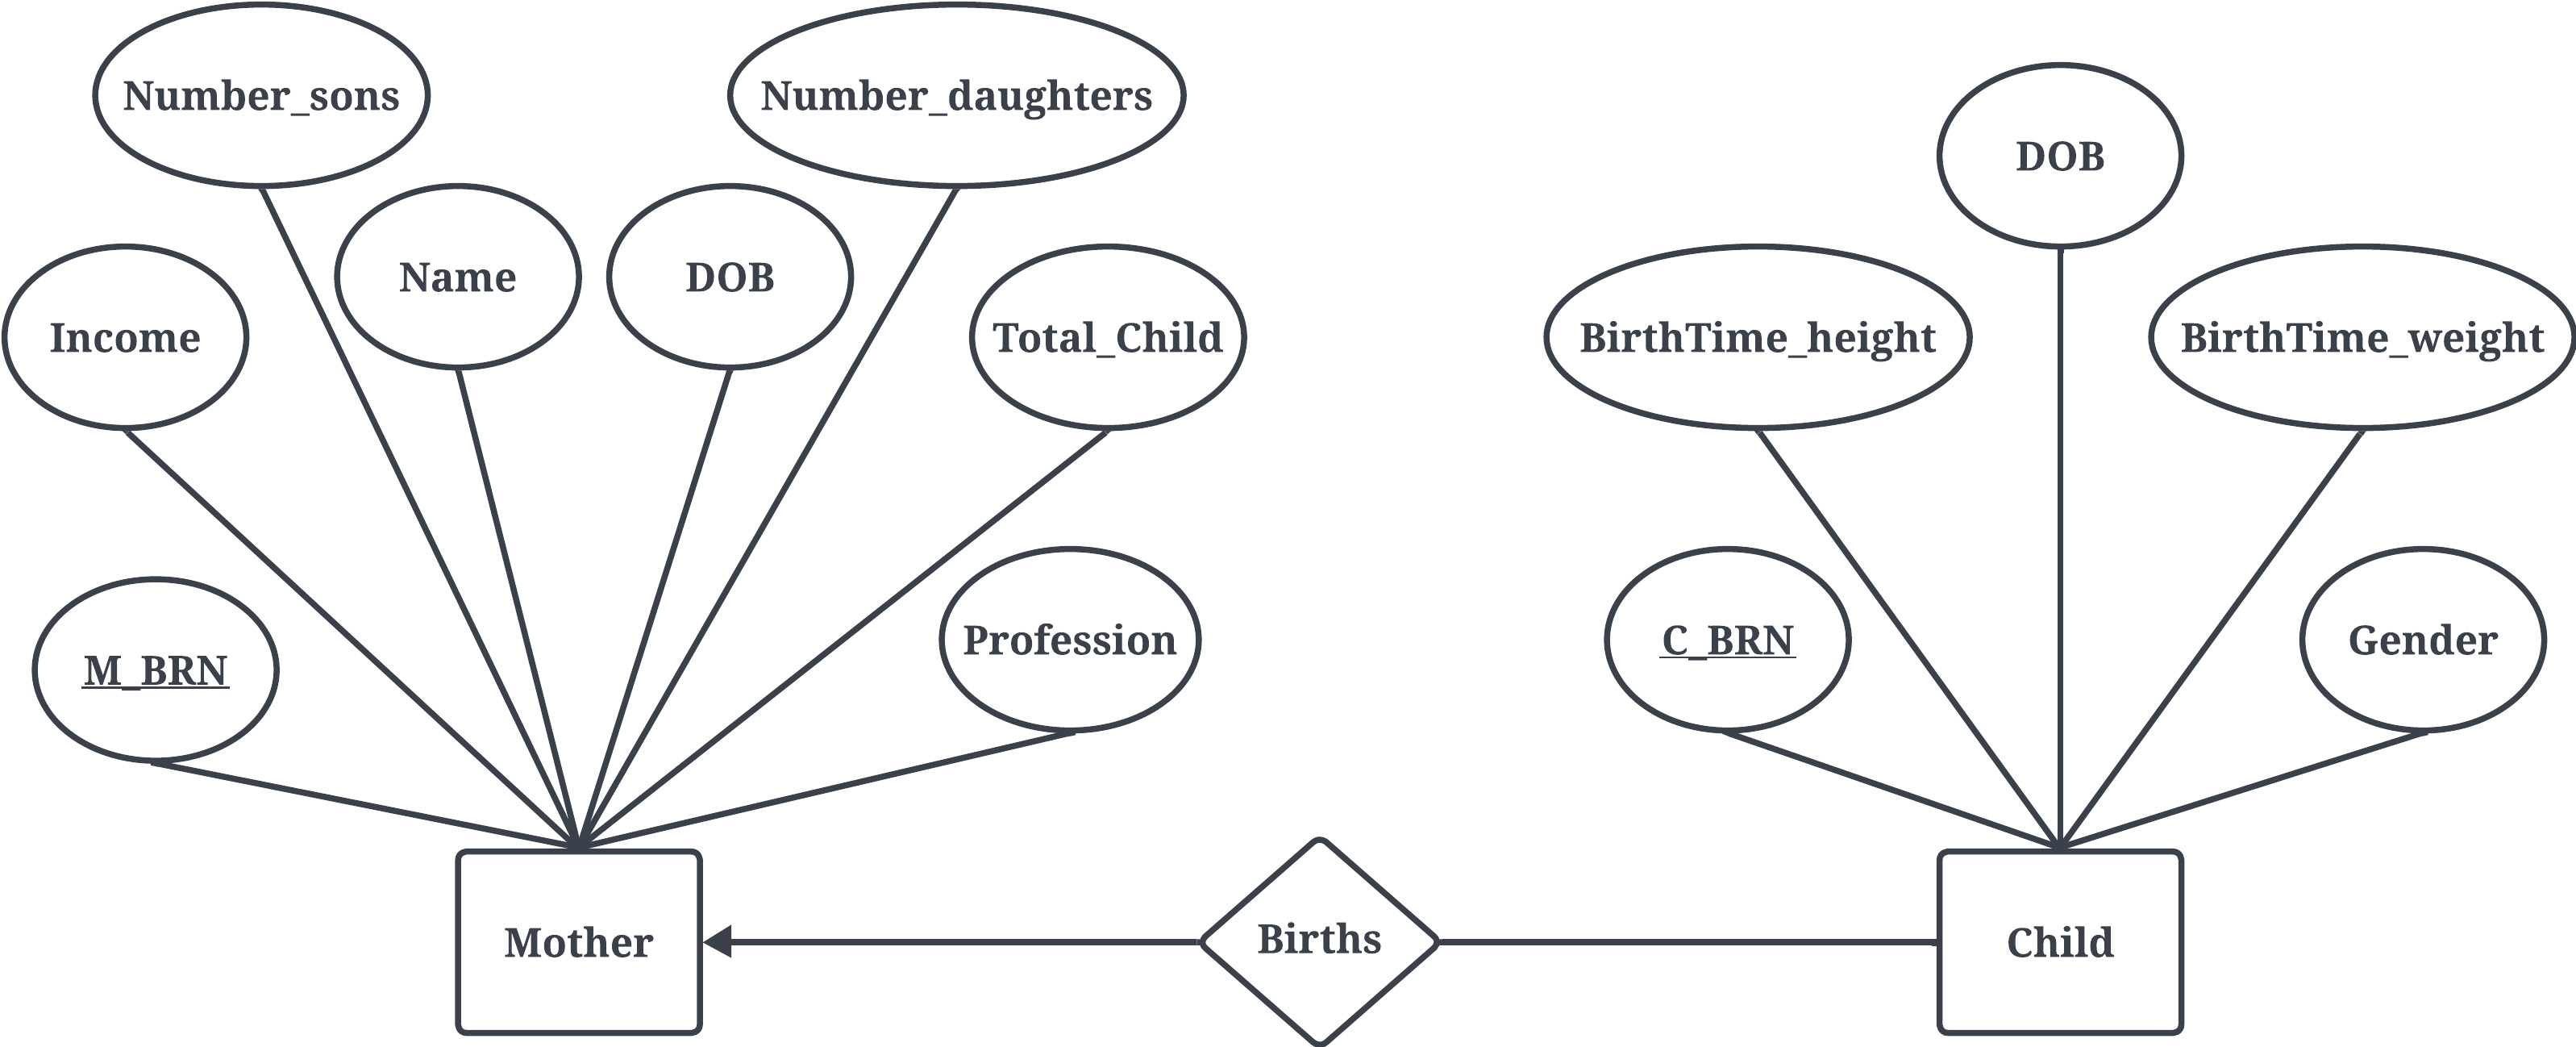
\includegraphics[width=1\linewidth]{Q2.jpeg}
    
    
\end{figure}

\section{\textbf{\uline{Q2 - Relation Schema:}}}
Mother(\uline{M\_BRN}, Name, Number\_sons, Number\_daughters, Total\_child, DOB, Profession, Income)

Child(\uline{C\_BRN}, Name, DOB, BirthTime\_height, BirthTime\_weight, Gender, M\_BRN) 
\\
\\
\section{\textbf{\uline{Q3 - ER Diagram (Chen Notation):}}}
\begin{figure}
    \centering
    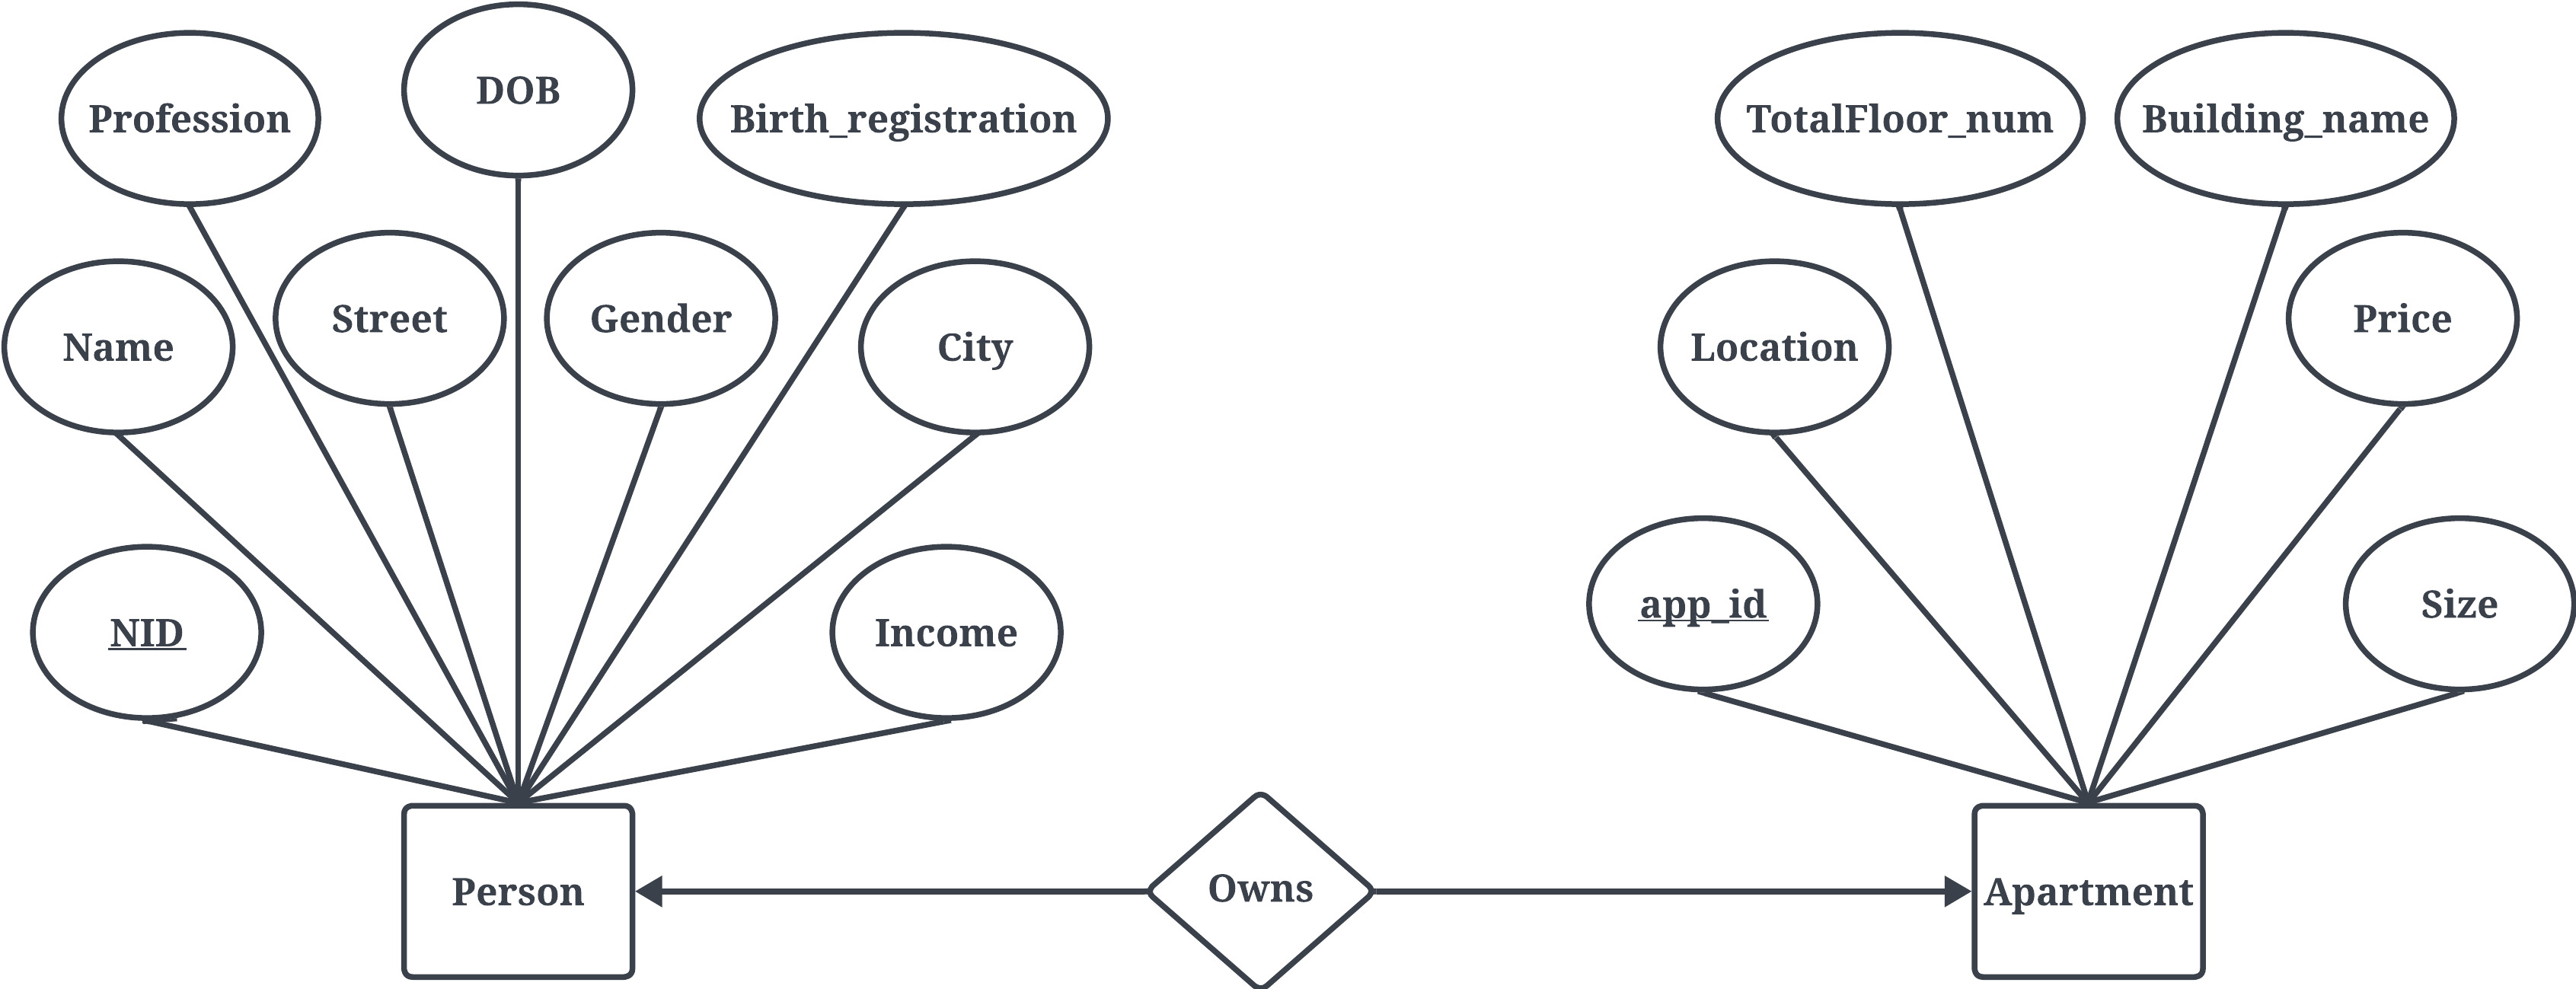
\includegraphics[width=1\linewidth]{Q3.jpeg}
\end{figure}

\section{\textbf{\uline{Q3 - Relation Schema:}}}
Apartment(\uline{App\_id}, Size, Building\_name, TotalFloor\_num, Location, Price)

Person(\uline{NID}, Name, Gender, DOB, Profession, Income, Street, City, Birth\_registration, App\_id)

\end{document}




